One of the main purposes of the patent processor project is to provide
a usable database of relevant patent data. This database should facilitate
the retrieval of patent records, citations, inventors, lawyers, assignees,
and other patent-related data. The linked nature of these types of
records suggests that a relational database model would be most suited
to the data, which motivated the decision to model patent data in
SQL. SQL, or Structured Query Language, is a language designed for
managing data held in a relational database.

Because the majority of the data processing pipeline is written in
Python, it is hard to integrate otherwise easy-to-use SQL code. There
are multiple flavors of SQL -- among them, SQLite and MySQL. SQLite
simplifies local development because the whole database is represented
as a single efficiently-sized file that can be copied, moved and manipulated
much like a traditional file. However, it is hampered by a lack of
support for more complex SQL features, and has poor support for concurrent
users (e.g. multiple processes attempting to access the same database).
MySQL offers advanced SQL features (such as \verb`LEFT OUTER JOIN`)
and scales to multiple users and large amounts of data much easier
than SQLite, but requires more specialized knowledge to use and access.
MySQL is more suited for production environments, whereas SQLite is
better for development. We want to be able to easily switch between
these two flavors of SQL depending on our purpose without having to
develop multiple branches of database integration.


\subsection{SQLAlchemy}

\begin{figure*}
\begin{lstlisting}
   number = ``%s''' % patent_number
result = connection.execute(query)
patent_id = result[3]
query = 'select * from assignee \
  where patent_id = ``%s''' % patent_id
connection.execute(query)
\end{lstlisting}
 \label{fig:sql-assignee} \caption{Finding assignees for a patent using traditional Python-SQL}
\end{figure*}


\begin{figure*}
\begin{lstlisting}
   filter_by(number = patent_number)
patent.assignees
\end{lstlisting}
 \label{fig:sa-assignee} \caption{Finding assignees for a patent using SQLAlchemy}
\end{figure*}


SQLAlchemy~\cite{sqlalchemy} is a Object Relational Mapper (ORM)
for Python that seeks to abstract away the differences between SQLite,
MySQL, and other SQL-based relational databases. The SQLAlchemy ORM
maps Python classes to an underlying SQL database such that the database
can be manipulated as though it were a native Python object. This
means that the object model and the database schema can be decoupled,
effectively removing the need for separate lines of development for
each possible database engine.

Database-related code written using SQLAlchemy is much cleaner and
easier to work with than the traditional, kludgy idioms. In the case
of SQLite, the normal Python module requires the user to excute strings
of SQL code: 
\begin{lstlisting}
   number = ``%s''' % patent_number
connection.execute(query)
\end{lstlisting}


Not only does this require the programmer to know SQL syntax, but
this paradigm leaves the database open to SQL injection, wherein unintended
and possibly malicious code is executed on the SQL database. For example,
here, we are operating on the assumption that the variable \verb`patent_number`
contains a valid patent number. It could actually contain the string
\verb`''; delete from Patent;--`, which would terminate the original
\verb`select` statement, delete all entries from the Patent table,
and then exit as though nothing had happened. To avoid such attacks,
it is necessary to sanitize all SQL strings to make sure they contain
valid and safe queries.

SQLAlchemy obviates the need to implement such verbose security methods.
The SQLAlchemy equivalent to the above query is:

\begin{lstlisting}
   filter_by(number = patent_number)
\end{lstlisting}


Immediately, we can see that this code is much simpler and cleaner.
When SQLAlchemy accepts string input, as with the \verb`patent_number`
variable here, it automatically escapes all significant characters
like semicolons and apostrophes, essentially nullifying the possiblity
of SQL injection attacks.

SQLAlchemy further simplifies the handling of foreign keys and complex
joins between tables, and can even implement these features over database
engines (such as SQLite) that do not normally have them. Consider
Figure 3 versus Figure 4.


\subsection{Limitations}

The nice features of SQLAlchemy come at a price. The higher level
interface to the SQL database requires a nontrivial amount of bookkeeping.
Foreign keys lookups and checks introduce a certain amount of overhead,
so when a process loops through a list of database items, multiple
SQL queries can be executed against the backend for each object if
the process asks for linked objects.

SQLAlchemy offers tools to help reduce the number of individual queries
sent to the underlying database, but there is an inescapable overhead
to using an ORM over the raw SQL.


\subsection{New Schema}

\begin{figure*}
\center 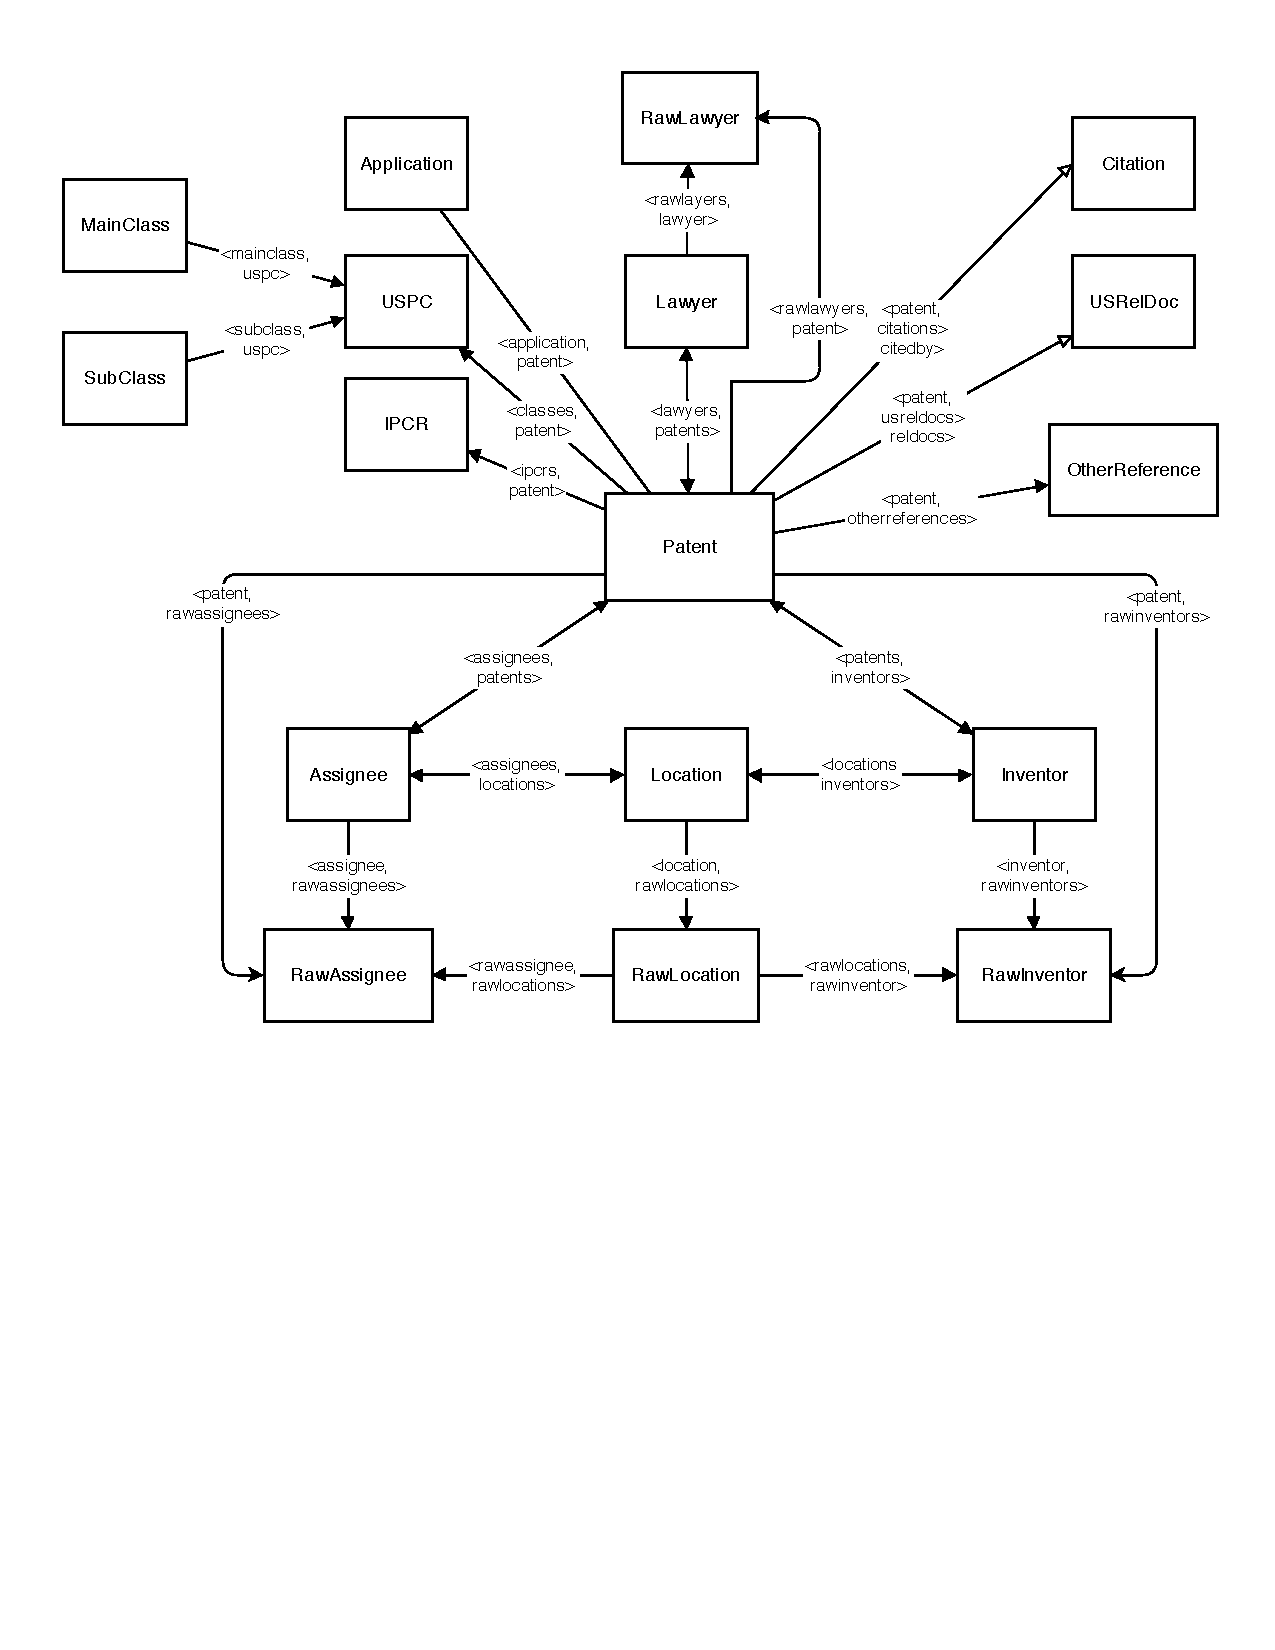
\includegraphics[width=0.6\textwidth]{figs/database-simplified}
\caption{High level view of new database schema}


\label{fig:newschema} 
\end{figure*}


We wanted to have a highly-linked database that would make it easy
for developers to access related information for a given set of patents.
The DVN schema, as described in the Appendix, does not take advantage
of foreign key relations, and places much manual burden on the user.
This was a primary motivating factor in our design, which is summarized
in Figure~\ref{fig:newschema}.


\subsection{Raw vs Processed}

If we examine the new database schema, for each of the \verb`inventor`,
\verb`lawyer`, \verb`location`, and \verb`assignee` tables, we
can see a ``raw'' version (e.g. \verb`rawinventor`) and a plain
version. The \verb`raw` tables contain the inventor, lawyer, location
and assignee records \emph{as they appear in the USPTO files}, which
means that the naming inconsistencies and misspellings are preserved.
These records are run through disambiguation methods of various degrees
of rigor, and the cleaned records are stored in the plain tables.
See below for a description of these disambiguation methods.

When the cleaned records are inserted, we link them to both the related
patent and the raw version using foreign keys in the database, so
it is simple to examine groups of related records. See Table~\ref{table:rawclean}.

\begin{table*}
\center %
\begin{tabular}{|l|l|l|}
\hline 
Table  & Access  & Value \tabularnewline
\hline 
Patent  & \verb`patent`  & US8434162 \tabularnewline
Inventor  & \verb`patent.inventors[0]`  & Thomas H. Stachler \tabularnewline
Raw Location  & \verb`patent.inventors[0].rawlocation`  & Deyton, OH, US \tabularnewline
Clean Location  & \verb`patent.inventors[0].location`  & Dayton, OH, US \tabularnewline
\hline 
\end{tabular}\caption{Accessing related raw and clean records. Note the spelling correction
in the clean record}


\label{table:rawclean} 
\end{table*}

